% !TEX root = fce.tex
% -----------------------------------------------------------------
% Filename  :	task4.tex
% Author    :	Carsten Hoppe
% Date		:	30. January 2017
% -----------------------------------------------------------------



\subsection{Introduction to the MIPS Enhancements}
\label{sec:introductionToEnhancements}

The aim of this exercise was to add multiple functionalities to a given CPU called „MIPS“. In the beginning there was no pipelining activated and several adjustments had to be maid. In this chapter each of the enhancements are introduced in principle and afterwards its concrete implementation is explained in detail.

For each enhancement a corresponding assemble instruction file was adapted and its execution was carefully observed. Only one enhancement at a time was changed at a time to reduce the space of errors that need to be handled at once.


\subsubsection{Activating Pipelining}
\label{sec:activatingPipelining}
The first wanted improvement of the mips was the activation of pipelining. The following adjustments were made:

Exercise 3-3.3 gave a hint about the writing of data back into a register at a negative clock edge ``The register file must be read in decode stage and written in write back stage within a single cycle.'' TODO Footnote

\lstinputlisting[caption={WBatFallingEdge.txt}]{appendix/task3_change1_WBatFallingEdge.txt}

Afterwards conveniently predefined registers which could save and pass on memory instructions at each phase of the pipeline could be inserted by changing the code belonging to each of the registers at the ID (Instruction / Decode) phase, at the EX (Execution) phase, the MA (Memory Access) phase, as well as the WB (Write Back) phase.

\lstinputlisting[caption={ActivatingPipelineRegisters.txt}]{appendix/task3_change2_activatingPipelineRegs.txt}

In order to make sure that no mistakes occured and all steps were taken according to the modification plan precise testing had to take place. Small simple programs were executed and examined using GTKWAVE, a visualization tool for vhdl code executions. First, an assembler program which was perfectly executed by the mips before the adaptions was modified with additional nop commands after each execution command in the code. In fact we needed exactly three nop commands because we were using a 4 stage pipeline and the longest number of clock cycles that one command needed to wait was three clock cycles at this point. The reason is we wanted to mitigate data and control hazards and needed to make sure that the registers were running as expected without taking care of the issues of forwarding and stalling yet. 

Of course it was not the aim to add three nop operations after each instruction every time. But in the beginning this was the approach needed. Later on the goal was to let the mips add nops wherever needed automatically by sending a stalling signal.

\subsubsection{Installing Forwarding}
\label{sec:installingForwarding}

After making sure that pipelining was running the next step at hand was to install a forwarding logic which implements the following behaviour:
\cacheResultFigure{pictures/task3_lectureDescriptionOfForwarding}{FEC Slides, Diagram of Forwading Logic}{fig:picTask3_1}
\lstinputlisting[caption={HazardDetectionForwardLogic.txt}]{appendix/task3_change3_hazardDetectionForwardLogic.txt}

The aim was to let instructions that were using registers that were written to in one instruction step earlier use the calculated information directly out of the ALU instead of having to wait until the calculation was written back into a register at WB phase.
The same procedure applies to instructions that needed a calculated result 2 or 3 cock cycles later.
 
\subsubsection{Implementing Stalling}
\label{sec:implementingStalling}

We needed to implement the functionality of the processor to „freeze“ certain processing steps. If an access of a cache or a command like „load word“ takes more than one clock cycle then consequent instructions needed to wait for the corresponding time delay. 
Our implementation basically uses a new signal called „“TODO Insert StallingSignal name which is to be called whenever such a delay occurs. It has three consequences:

The PC (Program Counter) is kept the same. As long as the stalling signal is set to one no new commands will be passed on to the instruction registers of the EX phase. If a stalling signal occurs the instruction registers in EX phase are overwritten with a nop command. This nop will be passed on to next instruction registers like MA and WB.

\lstinputlisting[caption={BubbleInsertionExPhase.txt}]{appendix/task3_change4_bubbleInsertionExPhase.txt}

The stalling signal will remain activated until the command which called the stalling signal reaches the EX, MA, or WB phase. The phase in which the signal is deactivated again depends on the command. Load word for instance only needs a delay of one stalling command. Whereas other commands like conditional branches where the result of the instruction has an impact on the stalling time need more cycles.

Before finding this optimal solution a dead one was chosen before. We overengineered a bit by inserting a counter which simple counted down from 3 to 0. Until it was clear that the pipeline itself could be used as a counter to set the stalling signal back to one. Our lesson was: Program as few things as possible, use all the available things that you can!

Again at this point we wrote small programs that activated to behaviour that needed to be checked and varied the numbers of auxiliary nops inbetween ciritical instructions until the system was running quite well.

\subsection{Activating BRAM}
\label{sec:activatingBRAM}

The next big task was to use BRAM (Block RAM) instead of DRAM (Distributed RAM). DRAM was more suitable as memory for the single cycle CPU, because BRAM has clocked outputs. Using BRAM introduces another pipelining step and would have been a disadvantage for a single cycle CPU. But in our case, with pipelining avticated, can be used in an efficient manner. If the mips were running on a FPGA then of course BRAM has the advantage that normally more resources are available.

The DRAM was turned into BRAM by commenting out the corresponding rising\_edge(clk) and falling\_edge(clk) comnmands in the bram.vhd file and started working on the issues of having to deal with an additional pipelining step. It turned out that all commands were read into the IF/ID phase one clock cycle later. This behaviour is shown in figure \ref{fig3-5}. The code that was executed was consisting of three nop operations followed bei a JAL command. The PC of the 4th command, JAL, ist 12. The three nops have PCs 0,4 and 8. The upper red marking demonstrates the delay of 2 clock cycles after the PC was set to the value of 12. Before within the single cycle mips without BRAM it only took one clock cycle for an instruction to appear in the ID phase. The old delay is represented by the green marking below the first one.

\begin{figure}[ht]
	\centering
  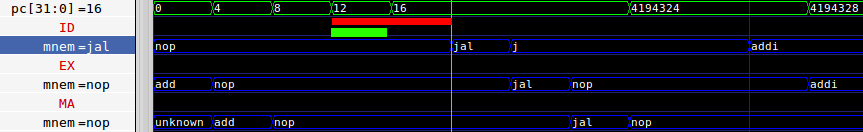
\includegraphics[width=1\textwidth, height=10cm, keepaspectratio]{pictures/task3_delayOfPCInstruction}
	\caption{Delay of PC instruction after 3 nops one JAL command}
	\label{fig3-5}
\end{figure}


%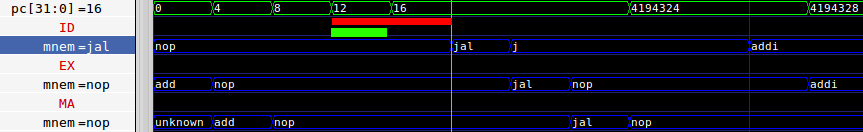
\includegraphics[width=15cm,height=10cm,keepaspectratio]{pictures/task3_delayOfPCInstruction}


%\cacheResultFigure{pictures/task3_delayOfPCInstruction}{Delay of PC instruction after 3 nops one JAL command}
	
Our control logic has to be adapted to the fact that now 4 nops had to be inserted instead of just three and also the program counter had to be frozen accordingly.
The PC freezing logic had to receive the instruction commands as early as possible. Therefore the logic needed to check the opcode of the instruction even before it was written into the first ID register. This way the system could understand when the program counter needs to be kept the same. Inserting nops after a branch or jump command occured in the ID register was not that much of a deal. The only big adaption was the addition of one stalling cycle more. Before the functionality basically was: If a jump or branch command occurs, stall until it reoccurs in MA phase, then set it back to '0' again. Now we needed one more stalling cycle and needed to let the stalling signal be set to '0' if the branch or jump command occured in the WB phase. Unfortunately the control instruction registers were not passed onto the WB phase from the MA phase. Therefore we had to adjust the system and add additional instruction forwarding in the mips\_pkg.vhd file.


TODO insert Mips pkg instruction forward information.

\lstinputlisting[caption={FreezingPC.txt}]{appendix/task3_change5_freezingPC.txt}


\subsection{Additional Details - One Nop at the Beginning Needed}
After our logic was implemented and the test runs were successfull it was interesting to see that some odd behaviour occured at the beginning of the program. It might be important to mention this behaviour in order to clearify   the situation and make bug hunting easier. The first command that is processed by the modified mips is a nop command due to the initialized state.  But it turned out that the second command will be executed twice in a row. In order to bypass this strange behaviour we simply inserted a nop at the beginning of each asm program. The consequence was a doubled nop command, which has no impact on the program at all.

\subsection{Lessons Learned so Far}
Besides the normal lessons like 

\begin{itemize}
\item ``keeping code as simple as possible"
\item ``commenting code pays off''
\item ``divide and conquer problems''
\item ``do testing, testing and testing''
\end{itemize}

another very important lesson was to take into consideration that it takes more time to get things running if team members are using different versions of an operating system or even different operating systems themselves. For instance we had to adapt scripts for windows and linux computers and during some time had different simulation results on our computers, which later on dissvoled after cleaning up temporary files and folders. Still this was quite annoying and took time to dissolve. Reducing the realm of possible error can be a big advantage.


